\section{MPC WITH GAUSSIAN PROCESSES}
\label{S:dpc}

This section presents a data-driven predictive control approach for buildings using GPs.
Suppose that GP models of a building's power demand and zone temperatures are already developed, as discussed in the previous section.
The predicted power demand at any future time $t+\tau$ in a window of $N$ time steps starting from the current time $t$, for \(\tau \in \{0,\dots,N-1\}\), is given by Equation~\eqref{eq:dpc:prediction}.
The output at time \(t+\tau\) depends upon %\(x_{t+\tau|t}\)  which is a function of
the control inputs \(u_{t+\tau-m}, \dots, u_{t+\tau}\).
We next show the flexibility of using these models in different applications.

\subsection{Demand Tracking Control}

\begin{figure*}[t]
	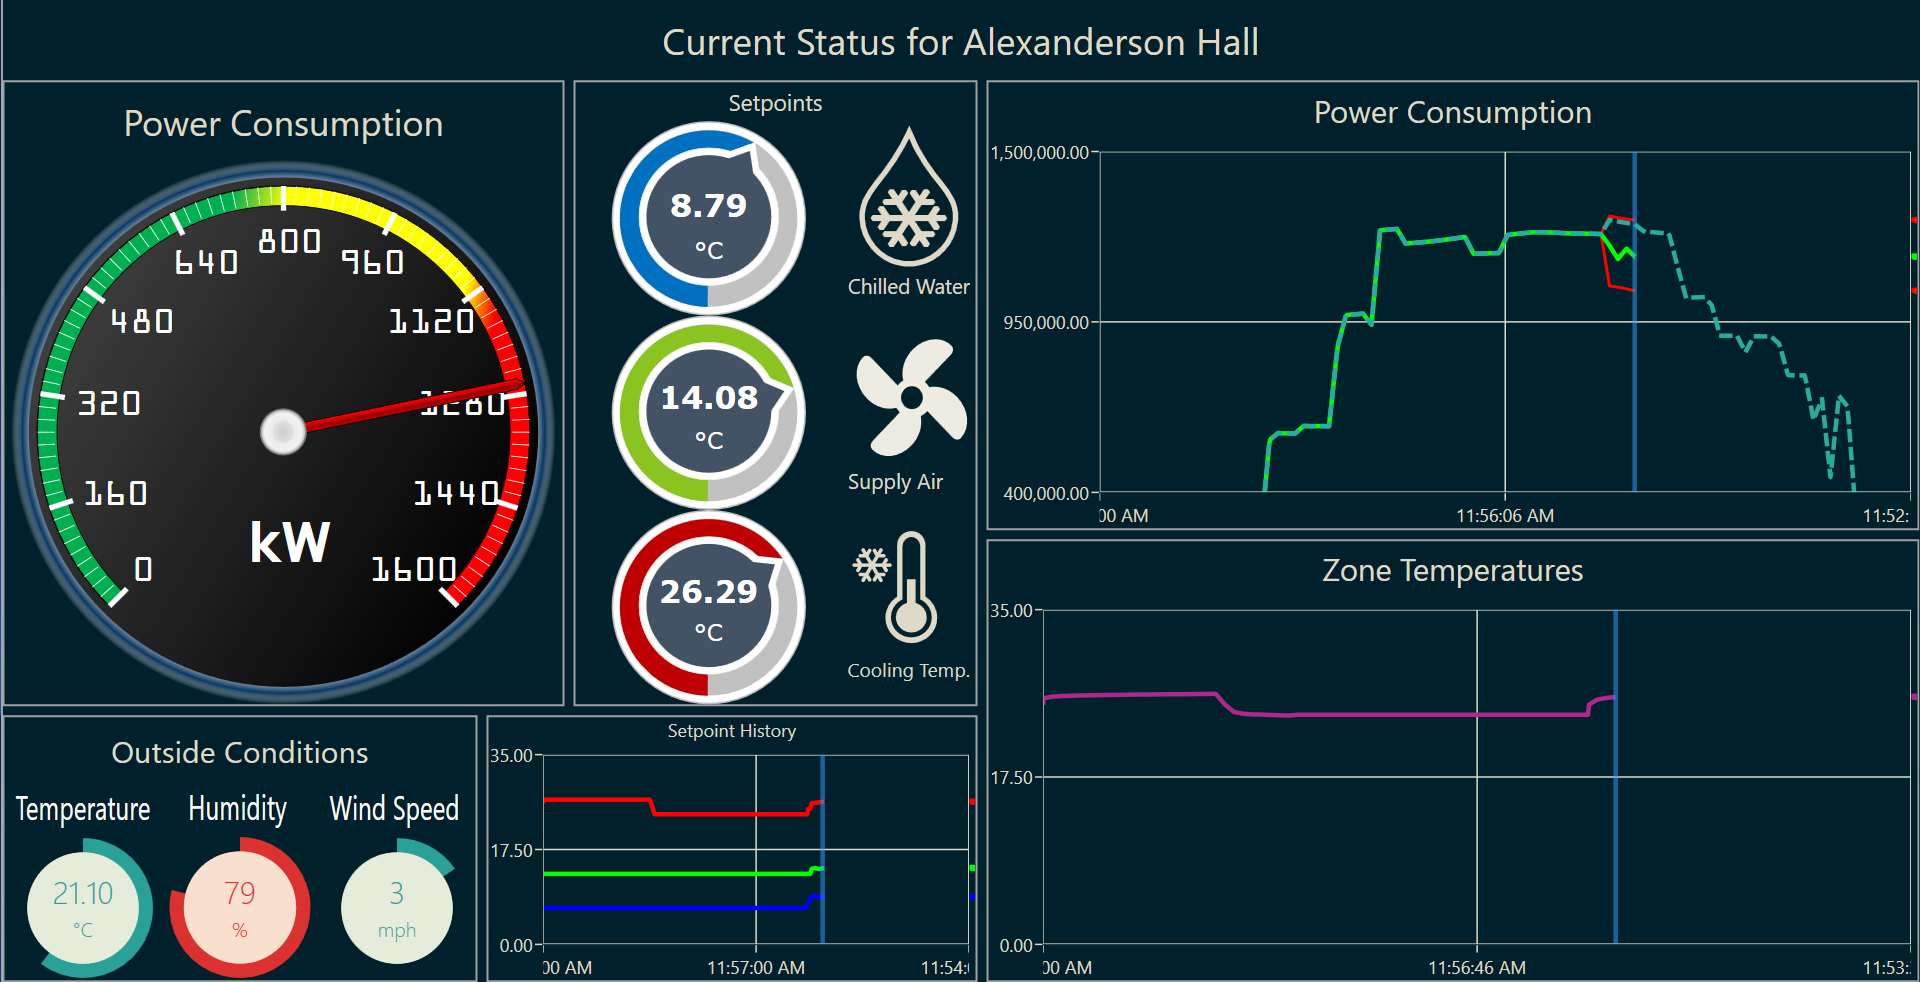
\includegraphics[width=\linewidth]{images/Dashboard-PowerTrack.png}
	\caption{Demand Tracking Control}
	\label{F:tracking}
\end{figure*}

This predictive control formulation fits demand response applications where a customer -- a building in this case -- must curtail its power demand by a certain amount from its baseline, or must track an Area Control Signal (ACS) sent from the grid operator.
For Demand Tracking Control we only require GP model \(\mathcal{M}_1\).
We are interested in solving the following optimization problem
\begin{align}
  &\minimize \sum_{\tau=0}^{N-1} (\bar{y}_{t+\tau} - y_{\mathrm{ref},t+\tau})^2 + \lambda \sigma^2_{y,t+\tau} \label{E:mpc:tracking} \\
  & 
    \begin{aligned}
      \text{subject to}\ \  & \bar{y}_{t+\tau} = \mu(x_{t+\tau}) + K_\star K^{-1} (Y - \mu(X)) \nonumber\\
      & \sigma^2_{y,t+\tau} = K_{\star \star} - K_\star K^{-1} K_\star^T \\
      & u_{t+\tau} \in \mathcal{U} \nonumber \\
      & \Pr(y_{t+\tau} \in \mathcal{Y}) \geq 1 - \epsilon \nonumber
    \end{aligned}
\end{align}
where the constraints hold for all \(\tau \in \{0,\dots,N-1\}\).
Here, \(K_\star = [k(x_{t+\tau}, x_1), \dots, k(x_{t+\tau}, x_N)]\), \(K_{\star \star} = k(x_{t+\tau}, x_{t+\tau})\). %, and $K$ is the covariance matrix with elements \(K_{ij} = k(x_i, x_j)\).
The signal $y_{\mathrm{ref}}$ is a reference power demand trajectory the building should follow as closely as possible.
The last constraint is probabilistic, which states that the building's power demand must stay inside a set $\mathcal{Y}$ with a probability of at least $1 - \epsilon$.
For instance, this constraint can control the quality of tracking the reference $y_{\mathrm{ref}}$.

We solve the optimization problem~\eqref{E:mpc:tracking} to compute optimal \(u_{t}^*, \dots, u_{t+N-1}^*\), apply \(u_{t}^*\) to the system and proceed to time \(t+1\).
Although all the constraints in \eqref{E:mpc:tracking} are of analytical forms, the optimization can be computationally hard to solve due to the high nonlinearity and computational burden of the GP.
% For the case study in Sec.~\ref{S:casestudy} we choose a combination of a squared exponential and rational quadratic kernel which results in nonconvex problem.
We use the nonlinear solver IPOPT \cite{Waechter2009b} and the optimization modeling framework CasADi \cite{Andersson2013b} to solve \eqref{E:mpc:tracking}.

\subsection{Climate Control with Minimum Energy Usage}

\begin{figure*}[t]
	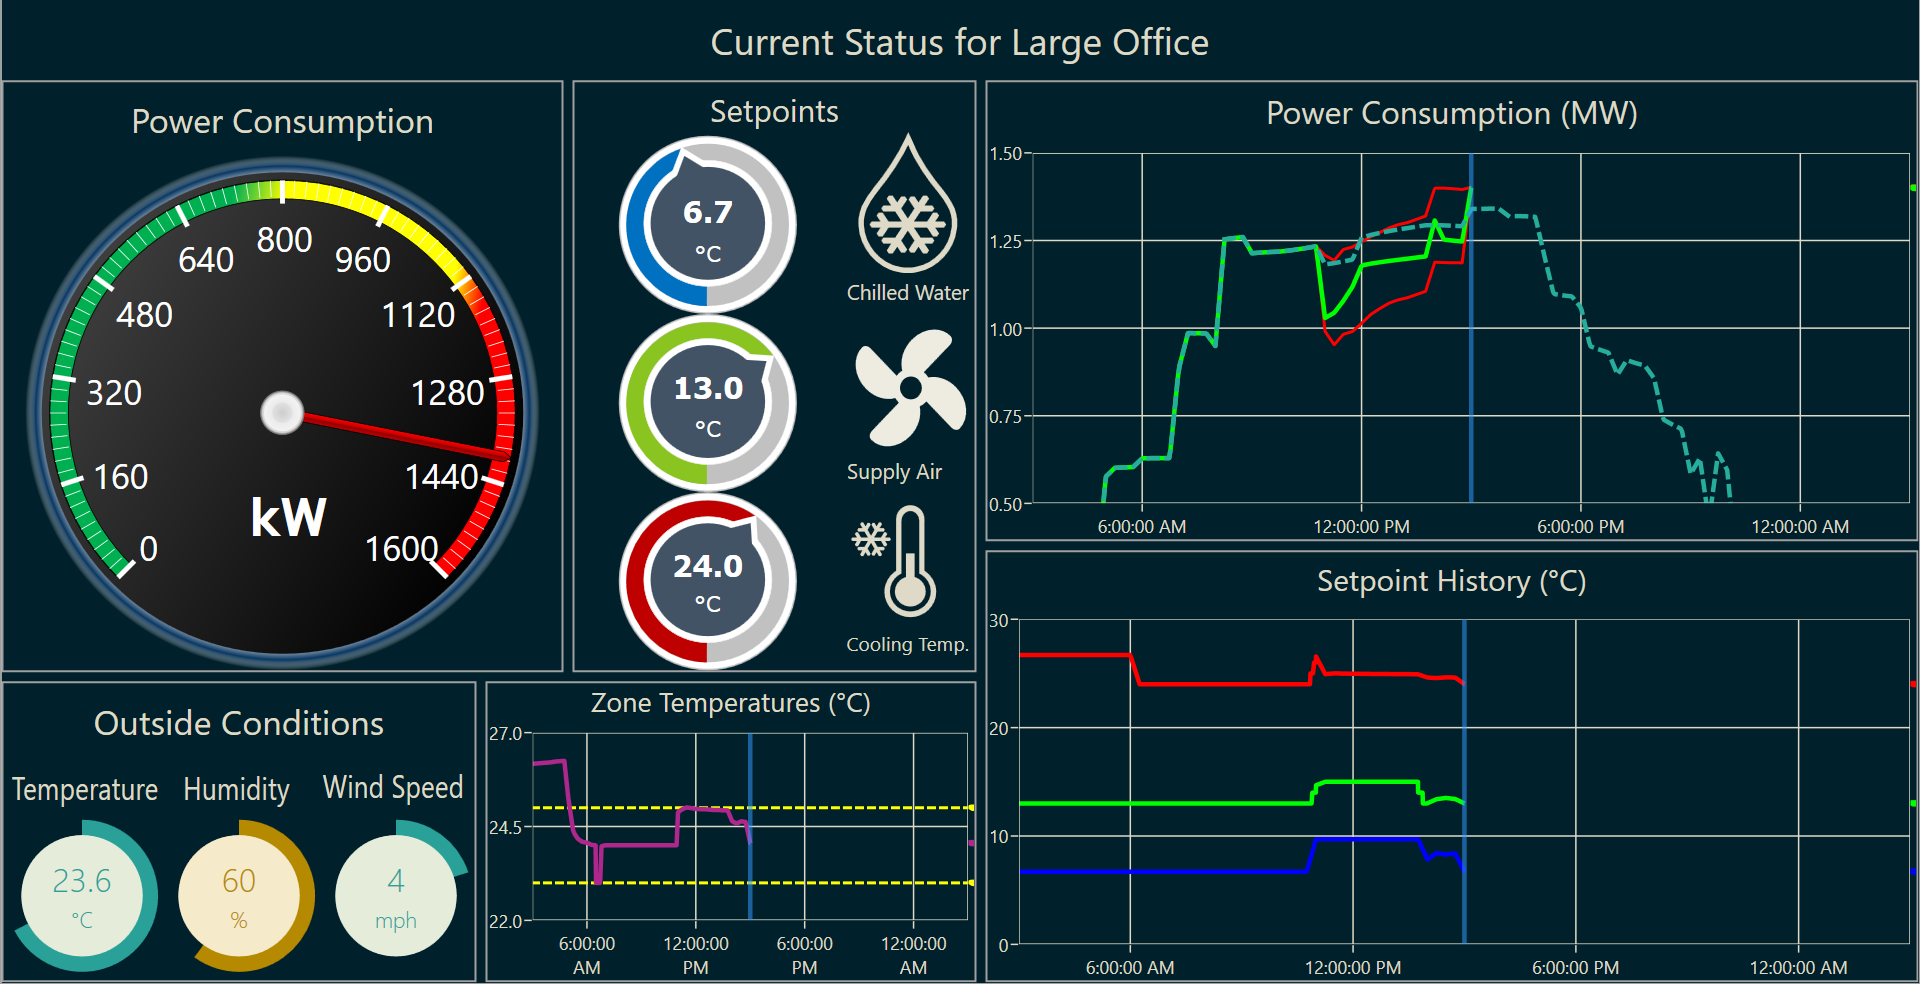
\includegraphics[width=\linewidth]{images/Dashboard-DR.png}
	\caption{Climate Control}
	\label{F:climate}
\end{figure*}

Other interesting objective for energy management is of minimizing energy usage while meeting thermal comfort constaints. In this example, we require both GP models \(\mathcal{M}_1\) and \(\mathcal{M}_2\).
Specifically, the model \(\mathcal{M}_2\) is used to enforce thermal comfort constraints in the optimization problem below:

\begin{align}
&\minimize \sum_{\tau=0}^{N-1} \bar{y}_{t+\tau} + \lambda \sigma^2_{y,t+\tau} \label{E:mpc:climate} \\
& 
\begin{aligned}
\text{subject to}\ \  & \begin{rcases}\bar{y}_{t+\tau} = \mu(x_{t+\tau}) + K_\star K^{-1} (Y - \mu(X)) \nonumber\\
\sigma^2_{y,t+\tau} = K_{\star \star} - K_\star K^{-1} K_\star^T
\end{rcases} \text{GP } \mathcal{M}_1 \\
& \begin{rcases}
 \bar{T}_{t+\tau} = \mu(x_{t+\tau}) + K_\star K^{-1} (Y - \mu(X)) \nonumber\\
\sigma^2_{T,t+\tau} = K_{\star \star} - K_\star K^{-1} K_\star^T \\
\Pr(T_{\mathrm{min}} \leq T_{t+\tau} \leq T_{\mathrm{max}}) \geq 1 - \epsilon \nonumber
\end{rcases} \text{GP } \mathcal{M}_2 \\
& \ u_{t+\tau} \in \mathcal{U} \nonumber
\end{aligned}
\end{align}
Here, \(\bar{y},\sigma^2_{y}\) denote the mean and variance of the GP \(\mathcal{M}_1\), and \(\bar{T},\sigma^2_{T}\) of the GP \(\mathcal{M}_2\). 
The goal is to optimize the inputs \(u\) that minimize the power consumption while maintaining thermal comfort with high probability. 
We again solve the optimization problem~\eqref{E:mpc:climate} to compute optimal \(u_{t}^*, \dots, u_{t+N-1}^*\), apply \(u_{t}^*\) to the system and proceed to time \(t+1\).

